\section{CLARA}
\subsection{Introduction}
The goal of the Clara project is to develop a framework which can be applied to a wide range of physics data processing applications for the CLAS12 experiments. The framework shall cover all stages of the physics data processing, including  physics and detector simulation, high level software triggers, reconstruction programs, physics analysis programs, visualization, etc.  

\subsection{The Problem Statement}
Physics data processing application development is a collaborative process. On one hand, it involves computer scientists developing framework and basic software components, while on the other hand, it calls for physicists to develop and implement specific algorithms, needed for simulation, reconstruction, calibration, etc.  In addition, there will also be a physicist developing the data analysis programs to produce the final physics results. Physics results productivity and quality depends on the number of the end user physicist, performing and/or crosschecking physics data processing stages. The unprecedented scale and complexity of the physics computing environment requires substantial software engineering skills from the end user physicist. As a result we have a reduced number of qualified data processing physicists, resulting in a poor physics outcome. 
CLAS12 computing environment must keep up with fast growing computing technologies. Taking into account a long lifetime of the physics data processing applications we must organize software in a way that permits including or discarding some of the software technologies in an easy way without major reorganization and/or redesign.

\begin{figure}[htbp] %  figure placement: here, top, bottom, or page
   \centering
   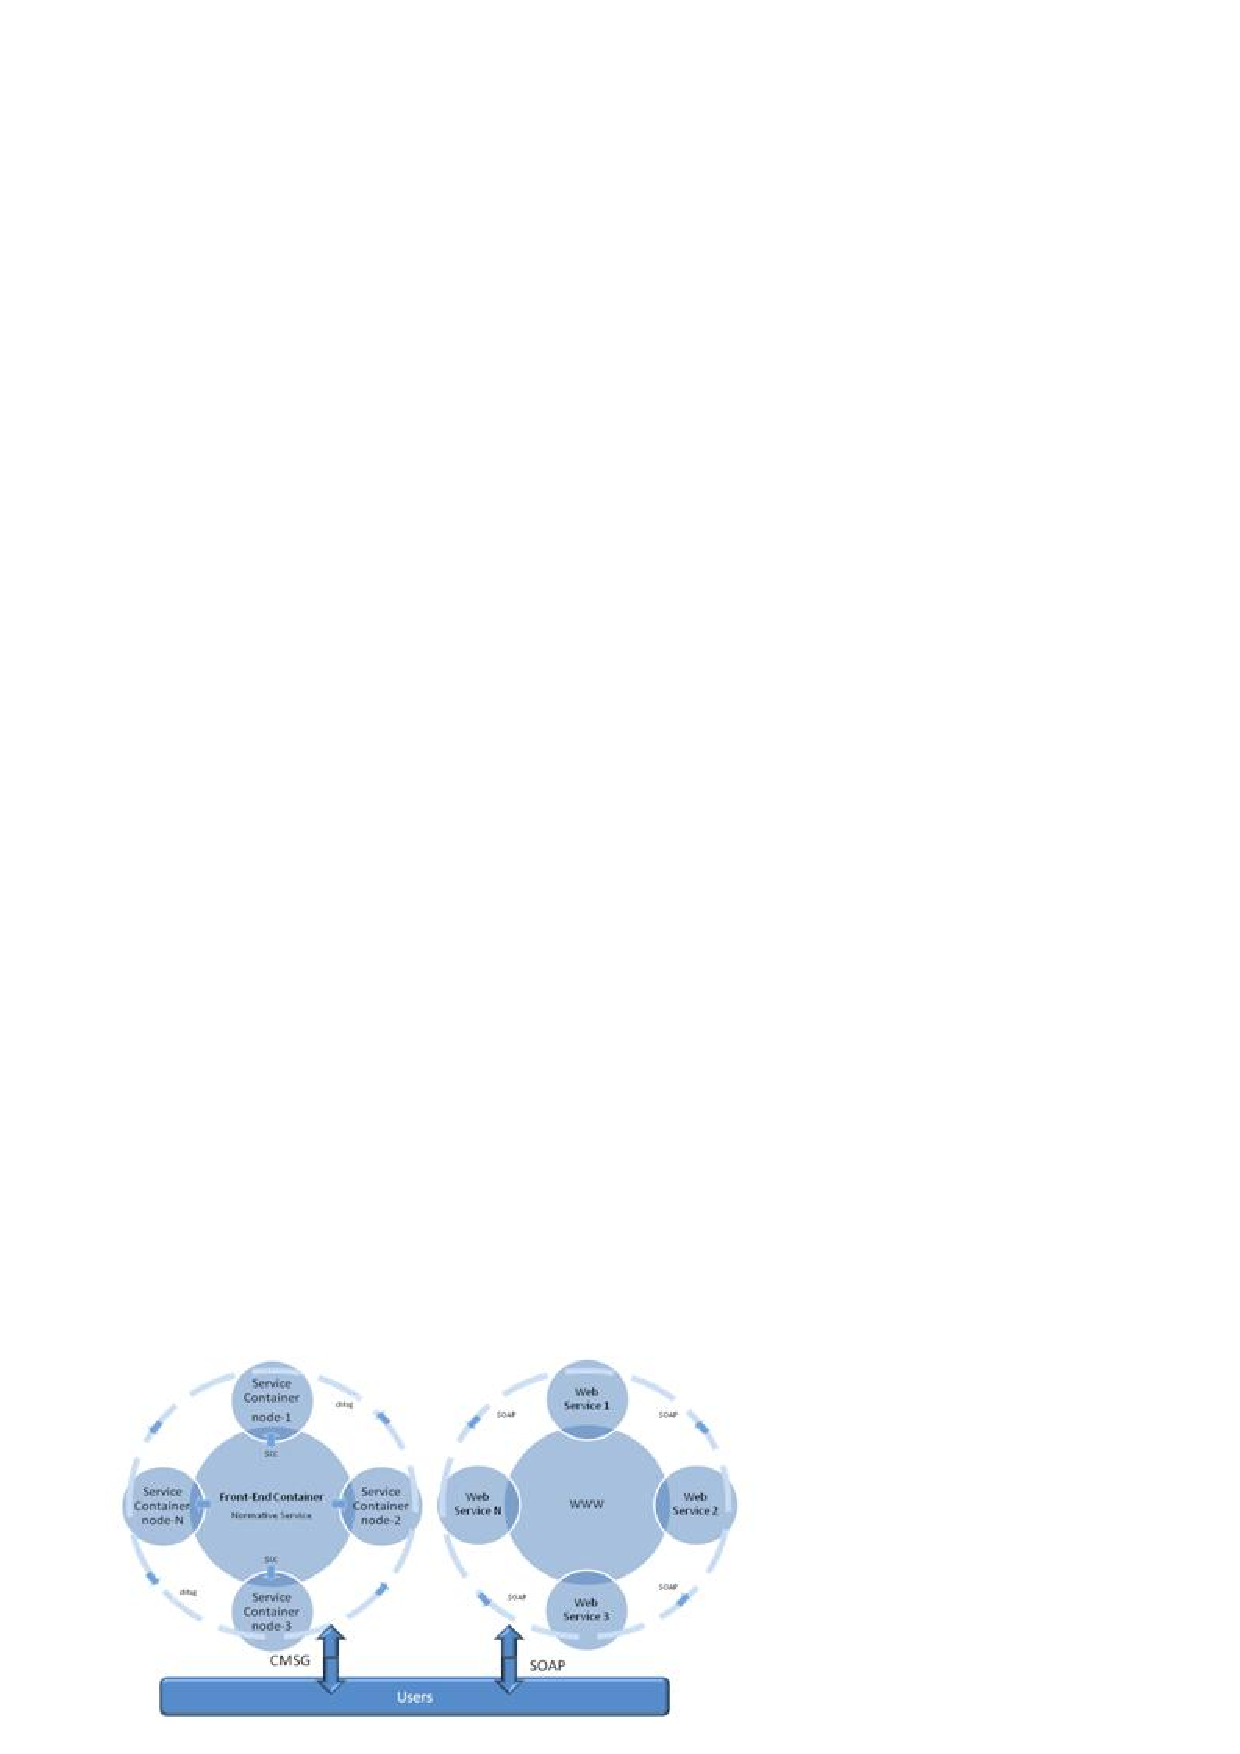
\includegraphics[width=4in]{CLARA/clara1.jpg} 
   \caption{Clara network distributed service platform. SCC: Service Communication Channel. cMsg: Publish-Subscribe messaging protocol. SOAP: Simple object access protocol.}
   \label{fig:clara1}
\end{figure}



\subsubsection{Physics data processing environment}

We have categorized three groups of people working with the framework. This categorization is not intended to be exclusive and it is a categorization of interaction rather than of people, since many people will belong to several groups.

A.	Framework developers. These people are responsible for the design, implementation and maintenance of the framework itself. 

B.	 Physics application software developers. This group of people will be required to have strong computing skills and more knowledge of the framework than what is required by the average physicist user.

C.	Framework users. These people are primarily interested in getting physics results. Using human machine interfaces they compose desired physics data processing applications and produce histograms, statistical distribution, etc.

Our goal is to widen the group C and make this group less dependent from the support of the A and B group people. 

\subsubsection{Design Requirements}
\begin{itemize}
\item Framework shall be simple to use and easy to learn.
\item Framework should be customizable to be able to adapt to the different data processing tasks.

\item Framework shall provide context sensitive help and assistance, with many real world physics data processing application examples.
\item Framework shall provide ready to use modules, encapsulating essential functionalities of the physics data processing system.
\item Modules shall be reusable and easily replaceable.
\item Physics data processing application design and implementation shall require a few or no programming skills.
\item Neither specific computing environment, nor compiling shall be necessary to build and run physics data processing application.
\item Framework shall provide graphical environment for physics data processing application development.
\item Framework shall be network distributed, and shall have temporal continuity.
\item The new system shall provide World Wide Web access to the framework for remote configuration and execution of the data processing applications. The necessary security considerations must be addressed. 
\end{itemize}
\subsection{SOA}


\begin{figure}[htbp] %  figure placement: here, top, bottom, or page
   \centering
   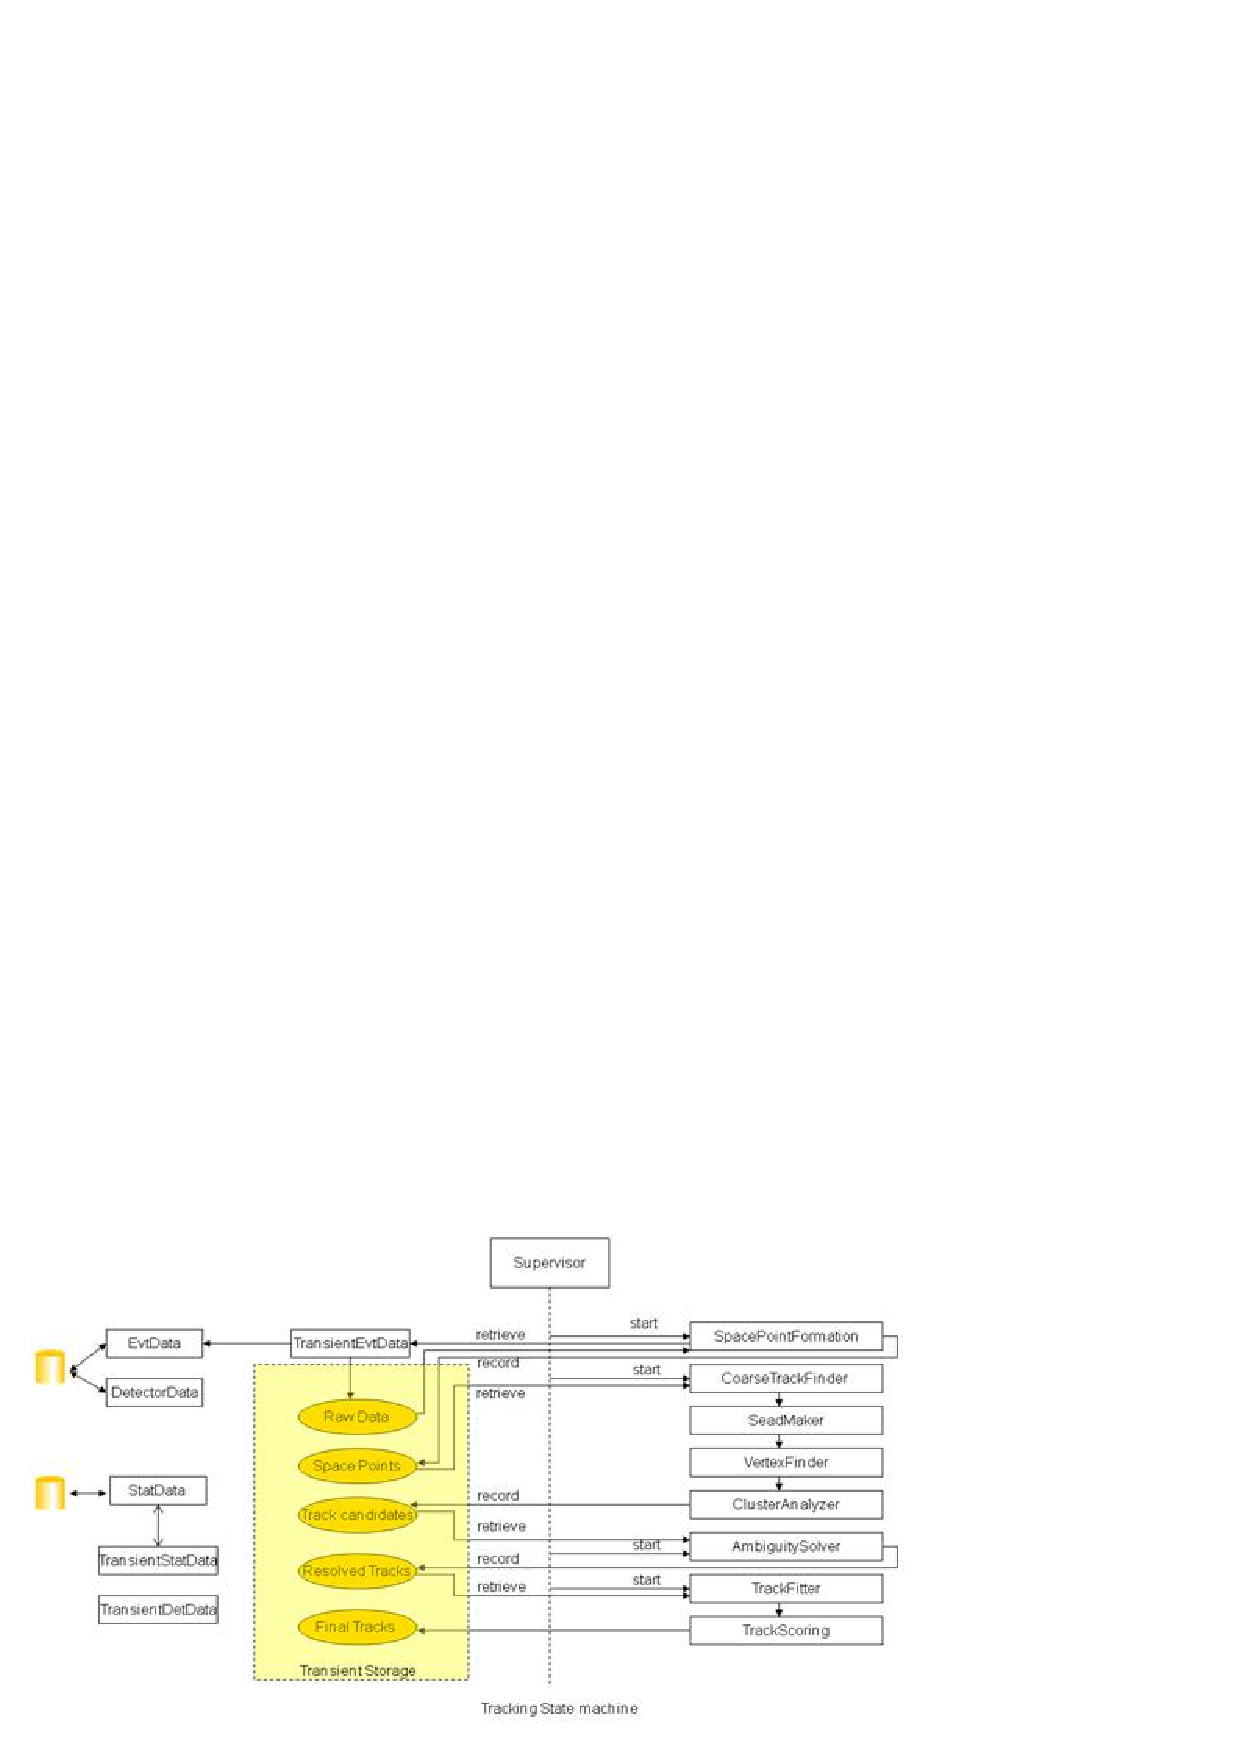
\includegraphics[width=4in]{CLARA/clara2.jpg} 
   \caption{Service decomposition of a hypothetical tracking application. Transient data is the memory resident EVIO format data. Ovals represent in memory data storage and rectangles services. Supervisor is the service that orchestrates the tracking application.}
   \label{fig:clara2}
\end{figure}

Clara identifies the physics data processing application as a composite application. A composite application is an application that is both assembled and orchestrated. An assembly is a process of combining together many different pieces into a workable unit, and an orchestration is making sure that those pieces work together collaboratively with one another to solve the given problem in a given scenario. Composite applications are known to be more efficient, robust and flexible. Composites of the software application know as software services are more specialized, easily maintainable, and easily replaceable and modifiable. Therefore software applications, composed of software services are extremely flexible, robust and adaptable to address different data processing needs. The SOA (service oriented architecture) provides the foundation for creating, deploying, maintaining and governing the software services. The Clara framework is the implementation of the SOA architecture        

\subsubsection{Design strategies}
Clara framework provides guidelines, policies and approaches for how physics data processing services are designed, deployed and managed. Clara services communicate with each other through message passing. Framework supports two distinct messaging protocols and transports: cMsg over TCP/IP and SOAP over HTTP. The services, using cMsg[1] proprietary publish-subscribe messaging protocol are designed to compose performance critical applications, and as usual are not requiring special security considerations. 

\subsubsection{Classification of the services}

Clara design guidelines are based on adopted design strategic decisions. In order to optimize service communications and service clustering Clara suggests separation between algorithm and data services. For example �cluster finder� is an example of the algorithmic service and �hits� in the calorimeter is a data service. Clara further categorizes data services into three categories: event, detector and statistical data services. Also standard data exchange format is used between services. EVIO [2] data format is used for data exchange between service.  
Clara supports flexible segmentation of the data processing application. In the very coarse level of segmentation a service is not different then a large monolithic software application. In this case Clara framework plays the role of a process manager and controller. Figure 2 illustrates an example of a tracking application service composition.

\subsubsection{Performance measurements}
Integration and coordination in real-time data and information from network distributed services will clearly carry performance penalties. It is also obvious that poor decomposition of the physics data processing application in terms of granularity can largely affect composed application performance.   

\begin{figure}[htbp] %  figure placement: here, top, bottom, or page
   \centering
   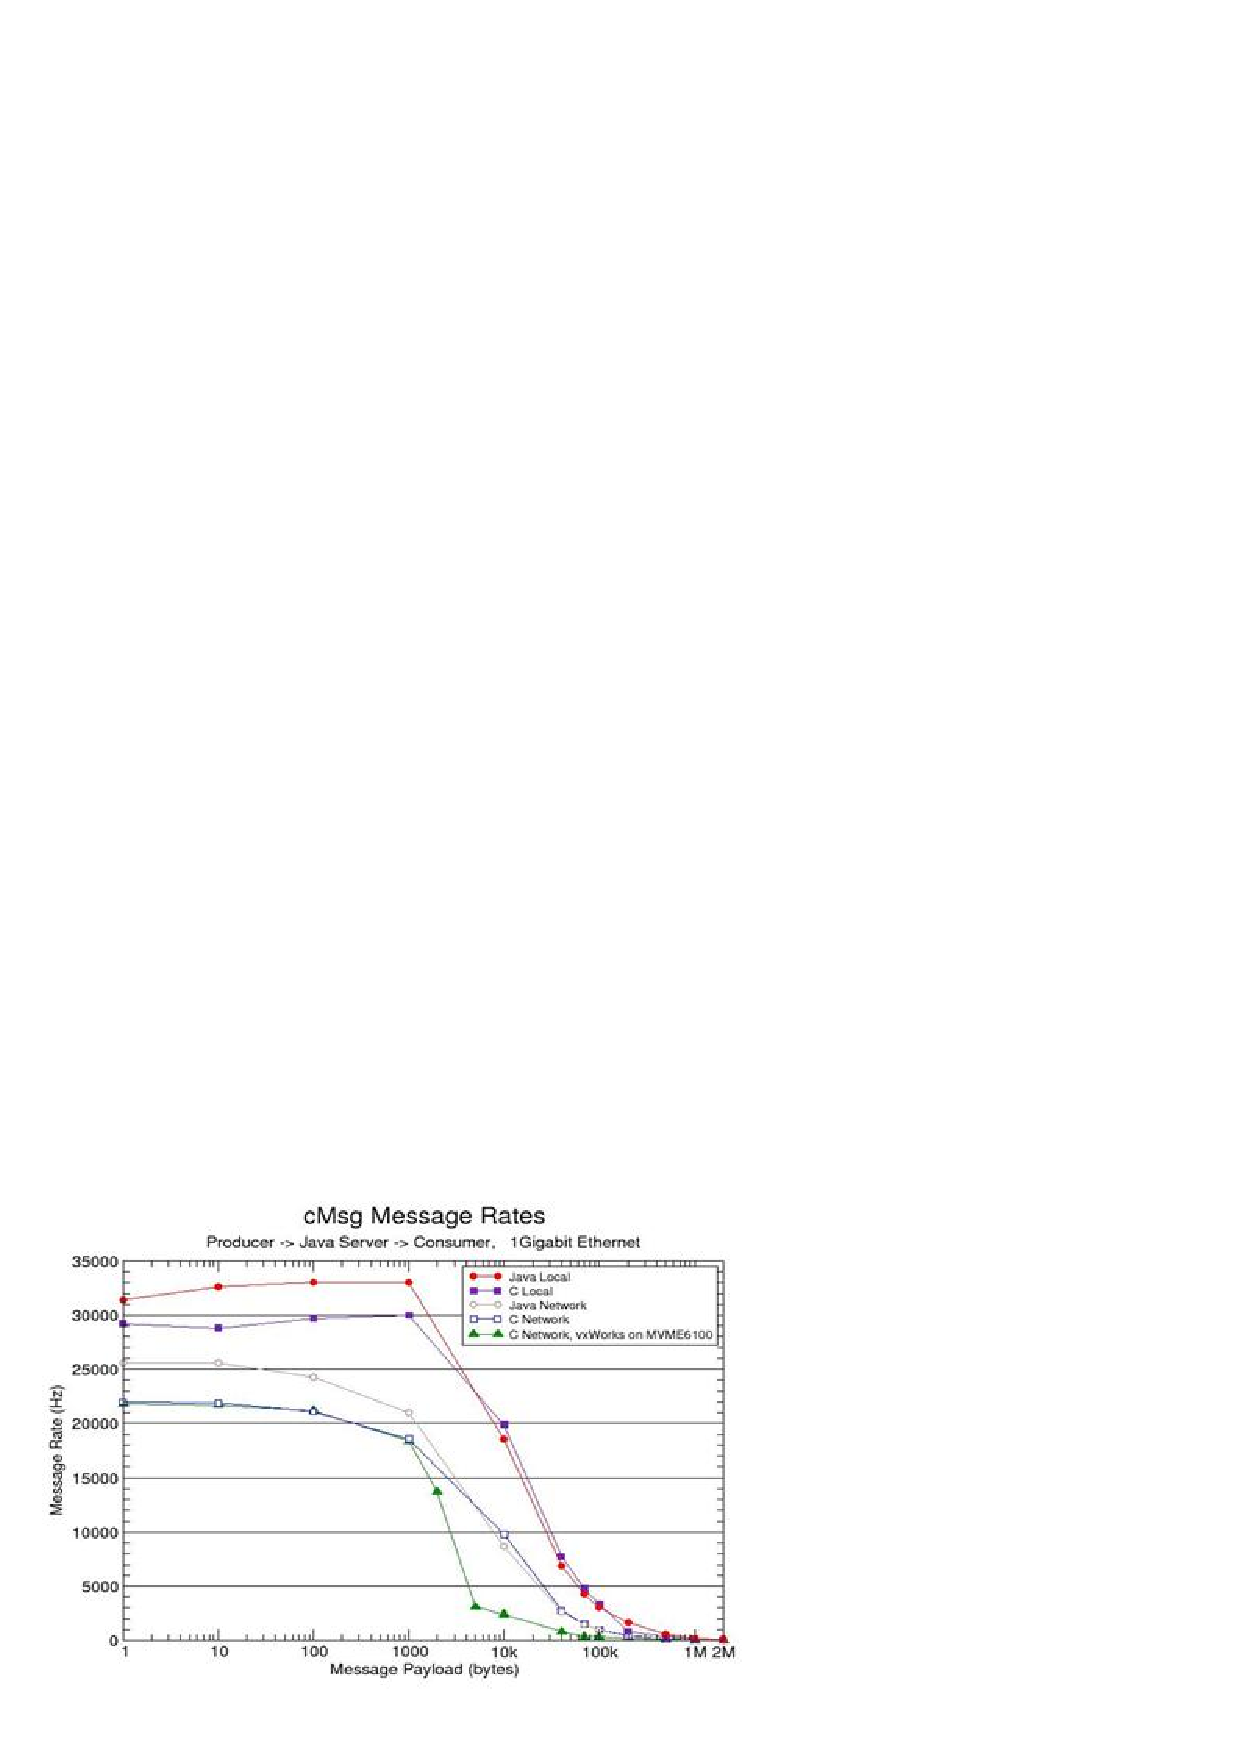
\includegraphics[width=4in]{CLARA/clara3.jpg} 
   \caption{cMsg measured performance.}
   \label{fig:clara3}
\end{figure}
 
\subsection{Web Services}

Clara web services are developed using J2EE (Java Enterprise Edition) JAX WS 2.0. Currently all the Clara cMsg services written in Java are also deployed as a Clara Web Services. Clara Web Services platform makes Clas12 services programmatically accessible over standard Internet protocols.




 


